%! suppress = EscapeUnderscore
%! Author = Leonardo Cruciani
%! Date = 29/03/2025

% Preamble
\documentclass[12pt]{article}

% Packages
\usepackage[top=1in, bottom=1.2in, left=1in, right=1in]{geometry}
\usepackage{amsmath}
\usepackage{upgreek}
\usepackage{graphicx}
\usepackage{subcaption}
\usepackage{wrapfig}
\usepackage{amsfonts}
\usepackage{hyperref}
\usepackage{longtable} % for 'longtable' environment
\usepackage{pdflscape} % for 'landscape' environment

\usepackage[backend=biber, style=authoryear]{biblatex}
\addbibresource{bibliography.bib}

\newcommand{\sym}[1]{\ifmmode^{#1}\else\(^{#1}\)\fi}


\author{Leonardo Cruciani}
\title{Replication of \\ Insider Trading and Innovation \\ by \textit{R. Levine et al.}}
% Document
\begin{document}
    \maketitle
    \section{Introduction}
    \label{sec:introduction}
    The paper examines whether legal systems that restrict insider trading,
    (i.e.\ trading by corporate officials or major shareholders on material nonpublic information)
    influence the invention of new technologies, as measured by patent intensity, scope, impact, generality, and originality.
    The ratio behind this study builds on~\textcite{fishman}, which shows that insider trading allows corporate insiders to exploit other investors,
    thus discouraging investment, and therefore, innovation.
    Moreover, innovative activities are particularly subject to the lack of trust, because generally more difficult to assess than more mainstream activities~\parencite{holmstrom}.
    \subsection{Dataset}\label{subsec:dataset}
    For a set of countries, the year when each country first enacts (i.e.\ passes) insider trading laws and enforces (i.e.\ when the firs violator is prosecuted) such laws is obtained from~\textcite{bhattacharya}.
    According to~\textcite{bhattacharya}, enforcement is more relevant than just enactment.
    The measures for innovations are 6 patent-based indicators, using industry-level data for each country, ranging between year 1976 and 2006, obtained from the European Patent Office's Worldwide Patent Statistical Database (PATSTAT).
    This dataset consists of 83200 industry-country-year observations.
    The indicators are:
    \begin{itemize}
        \item Patent Count: number of patents 
        \item Citation Weight: number of forward citations to patent filed 
        \item Top 10\% Patents: number of patents that become part of the top 10\% citation in their technology class 
        \item Patent Entities: number of patenting entities 
        \item General Innovation: degree of citations of the patents from other technology classes patents 
        \item Originality: degree of which the patents cite patents in other technology classes 
    \end{itemize}

    \section{Methodology}\label{sec:methodology}
    \subsection{Preliminary analysis}\label{subsec:preliminary-analysis}
For a first analysis, the data is aggregated to a country level.
The baseline regression equation is thus:
\begin{equation}
    Y_{ict} = \alpha_0 + \alpha_1 E_{ct} + \gamma X'_{ict} + \delta_c + \delta_i + \delta_t + \varepsilon_{ict},
\end{equation}
where the indices $(i,c,t)$ refer to, respectively, industry, country and year; $Y_{ict}$ is one of the six patent-based indicator, the $\delta$`s are country, industry and time fixed effects; $X_{ict}$ is a vector of controls, such as:
$ \log GDP, \log GDP/Population, Stock/GDP, Credit/GDP, Trade $, all obtained from the World Development Indicators and the Financial Development Infrastructure of the World Bank; and finally $E_{ct}$ is the insider trading law enforcement dummy: for each country, it is 0 if there are no insider trading laws enforced, and 1 otherwise.
The coefficient of interest for the treatment effect is thus $\alpha_1$.
The authors thus perform the regression using the Regression with Double Fixed Effects and Heteroskedasticity-Robust Standard Errors Stata package \texttt{reghdfe} and find that the enforcement of insider-trading laws is associated with a statistically significant, economically large and highly robust increase in each of the six patent-based indicators, ranging from $15$\% to $29$\%, as shown in table~\ref{tab:baseline}.
\begin{table}[h!]
    \caption{Author's baseline estimates, without and with controls}
    \label{tab:baseline}
    \centering
    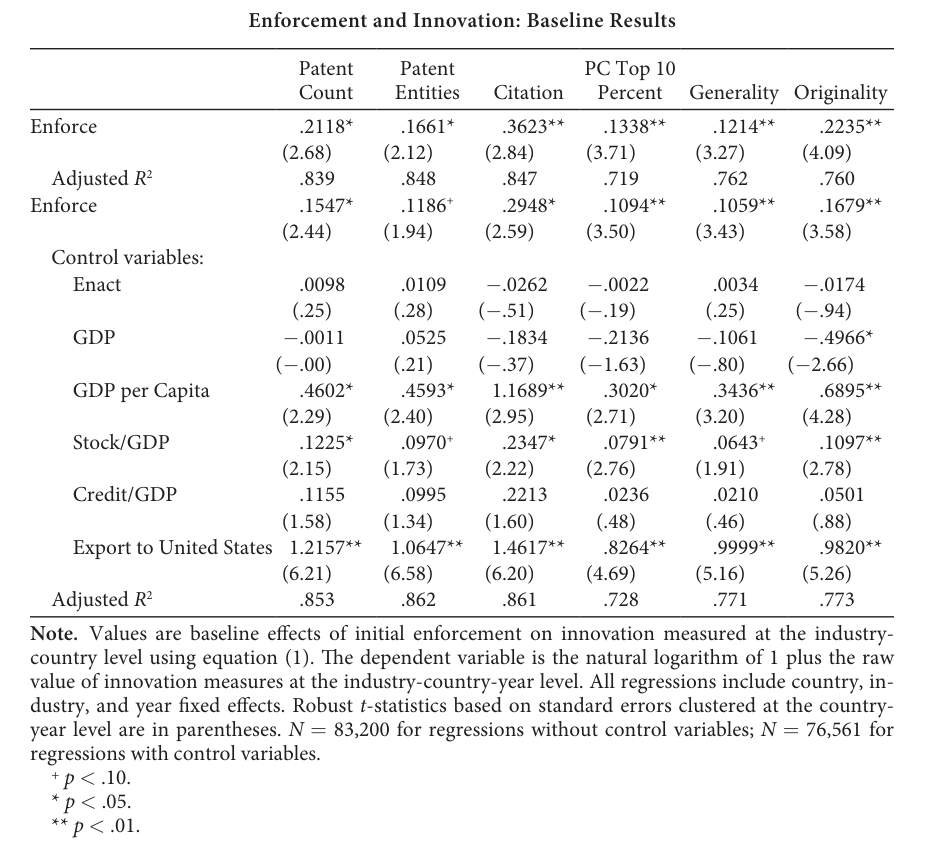
\includegraphics[width = 0.6\textwidth]{tables/baseline_orig}
\end{table}

\subsection{Industry level analysis}\label{subsec:industry-level-analysis}
The authors then proceed to evaluate the problem at industry granularity: they introduce an industry dummy $I_i$ to the baseline regression:
\begin{equation}
    Y_{ict} = \beta_0 + \beta_1 I_i E_{ct} + \lambda X'_{ict} + \delta_{ct} + \delta_{it} + \varepsilon_{ict},
\end{equation}
finding similar results to the baseline regression.

\subsection{Robustness and validation}\label{subsec:robustness-and-validation}
The authors perform various tests and robustness checks, including:
\begin{itemize}
    \item Check for omitted variable bias by including and excluding a large set of additional controls, composed of several indictors of securities-market reforms and policies toward international capital flows; an array of indicators of bank
    regulatory and supervisory policies; and enactment of patent laws, measures of intellectual-property-rights protection, property-rights protection more generally, and the effectiveness of the legal system.
    They find that including or excluding these controls do not alter the results.
    \item Do not find any pretrends in the patent-based measures of innovation before enforcement, based on graphical analysis.
    \item Find that the growth rates in innovation measures do not predict the enforcement of the laws, using a Hazard-Model estimation.
\end{itemize}

\subsection{Dynamic}\label{subsec:dynamic}
The authors study the behaviour of the innovation proxies in a $(-5,10)$ window around the enforcement year, implementing:
\begin{equation}
    Y_{ct}  = \alpha_0 + \sum_{\tau=-5}^{10} \alpha_{1,\tau} E_{c,t,\tau} +\delta_c +\delta_t + \varepsilon_{ct}
\end{equation}
They find a sizeable increase in innovation around the treatment year, while the control variables stay almost constant, as can be seen in figure~\ref{fig:dynamic_orig}.

\begin{figure}[h!]
    \centering
    \begin{subfigure}[b]{0.45\textwidth}
        \centering
        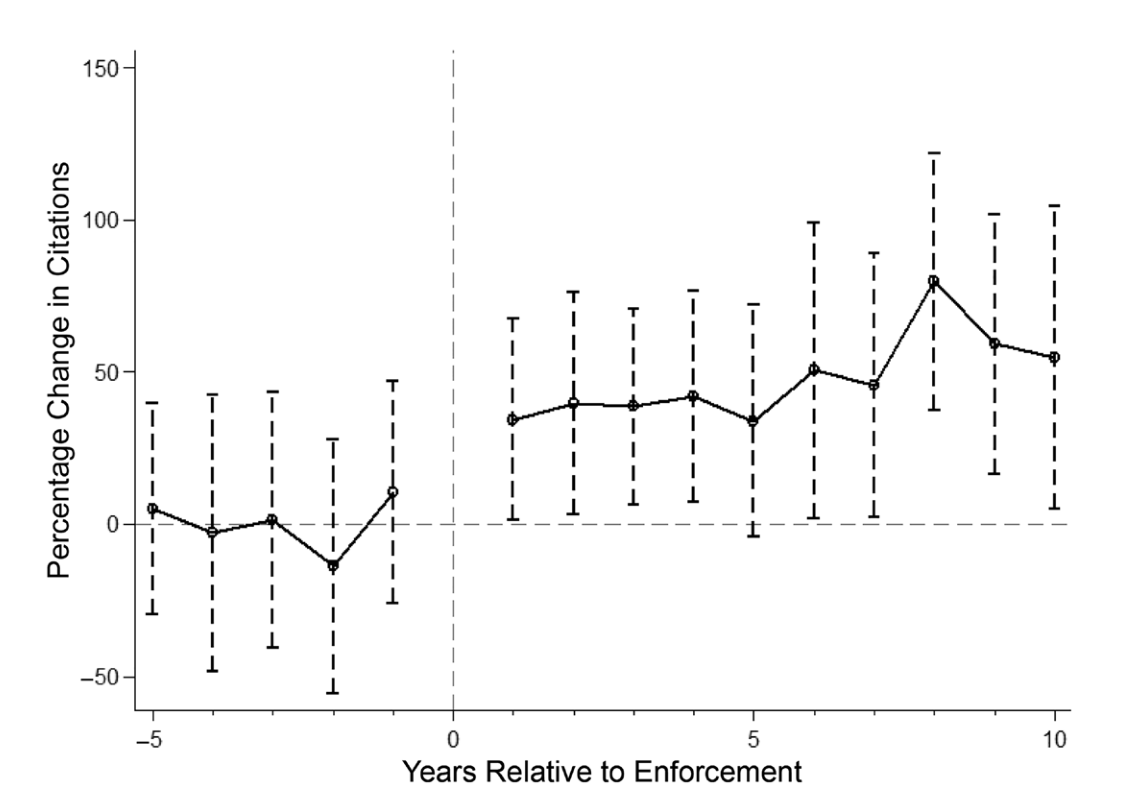
\includegraphics[width=\textwidth]{images/dynamic_orig_citations}
        \caption{Citation Weight}
    \end{subfigure}
    \hfill
    \begin{subfigure}[b]{0.45\textwidth}
        \centering
        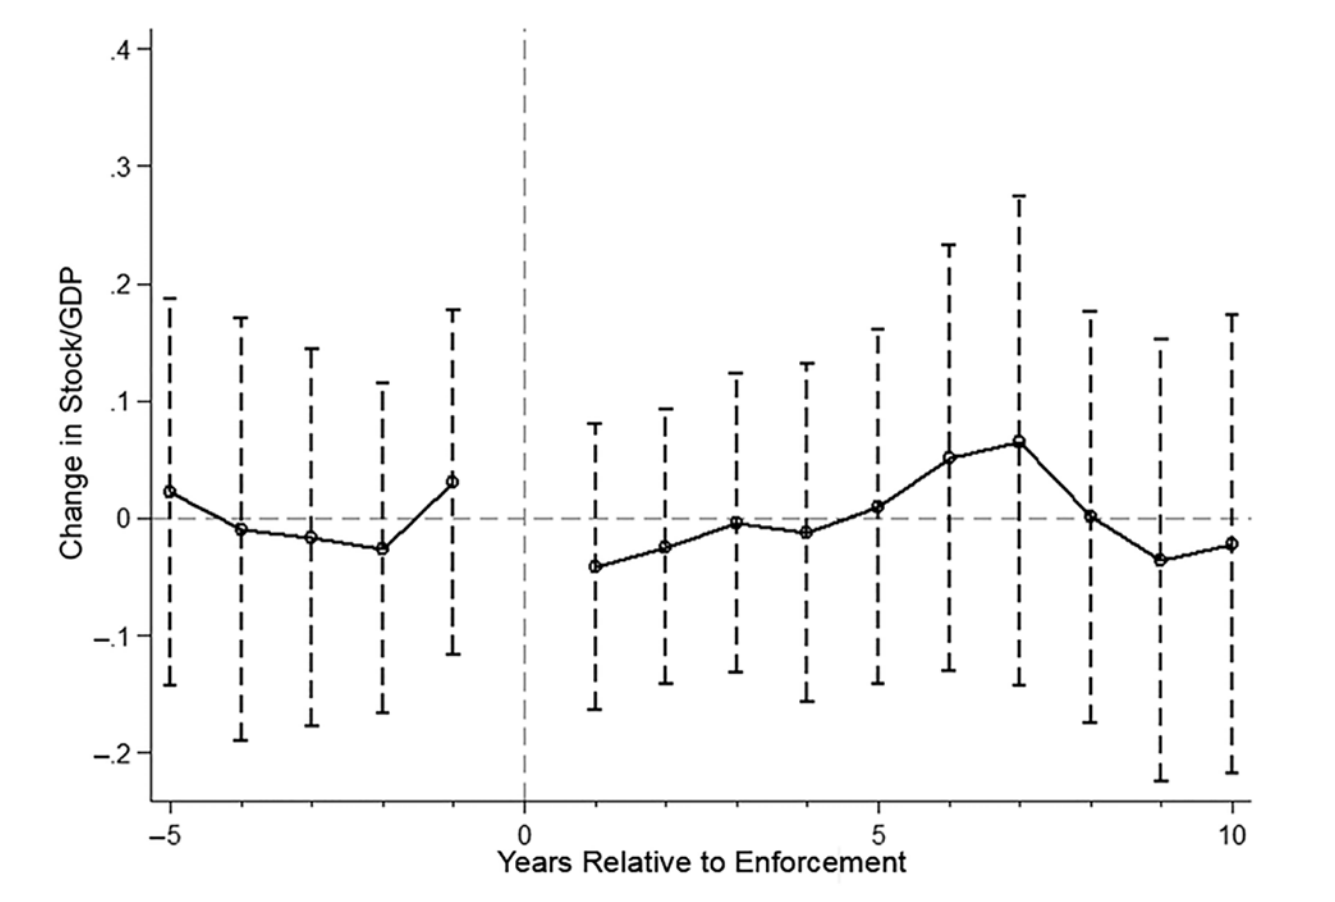
\includegraphics[width=\textwidth]{images/dynamic_orig_stock}
        \caption{Stock Market Capitalization}
    \end{subfigure}

    \vspace{0.5cm}

    \begin{subfigure}[b]{0.45\textwidth}
        \centering
        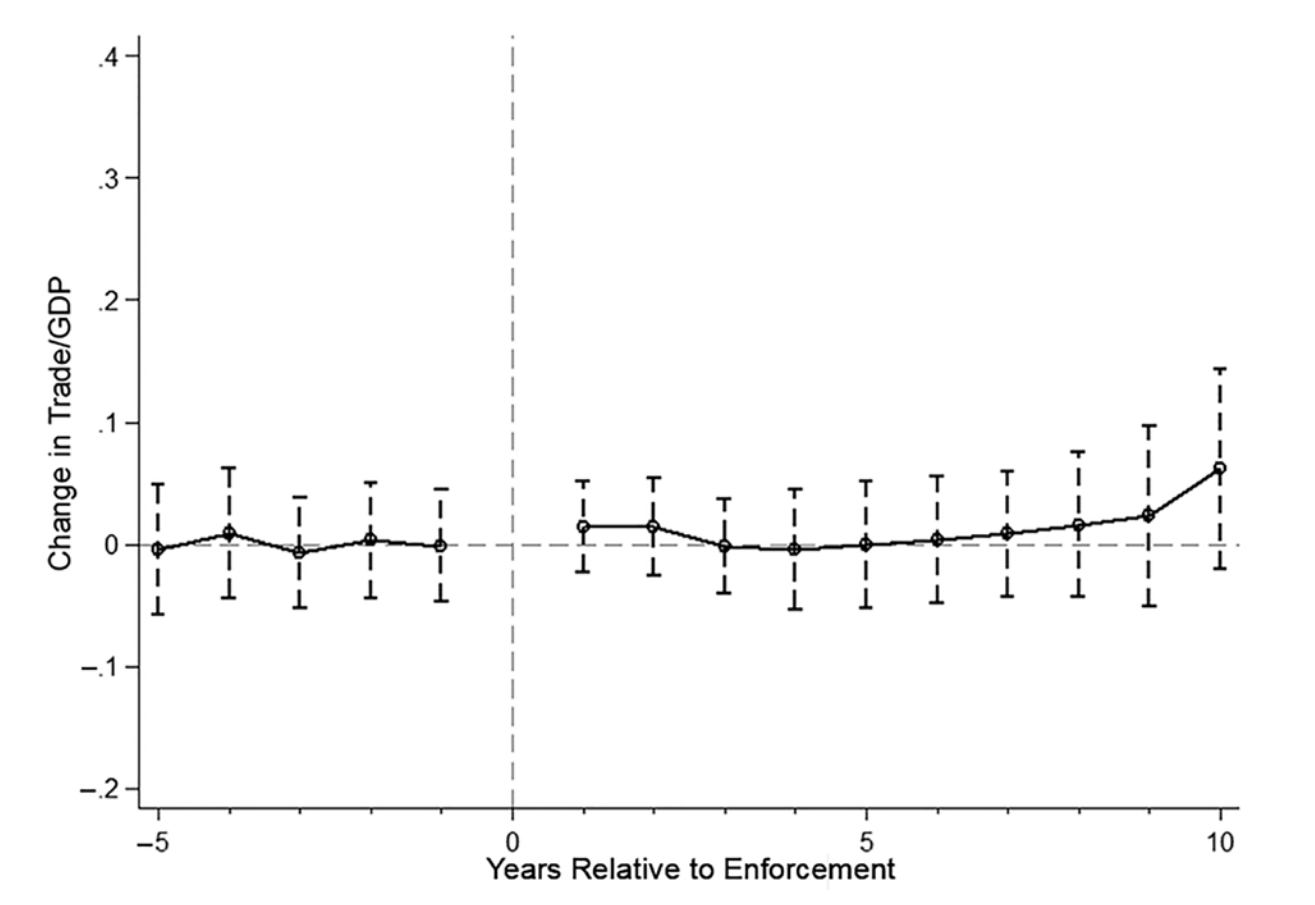
\includegraphics[width=\textwidth]{images/dynamic_orig_trade}
        \caption{Trade}
    \end{subfigure}
    \hfill
    \begin{subfigure}[b]{0.45\textwidth}
        \centering
        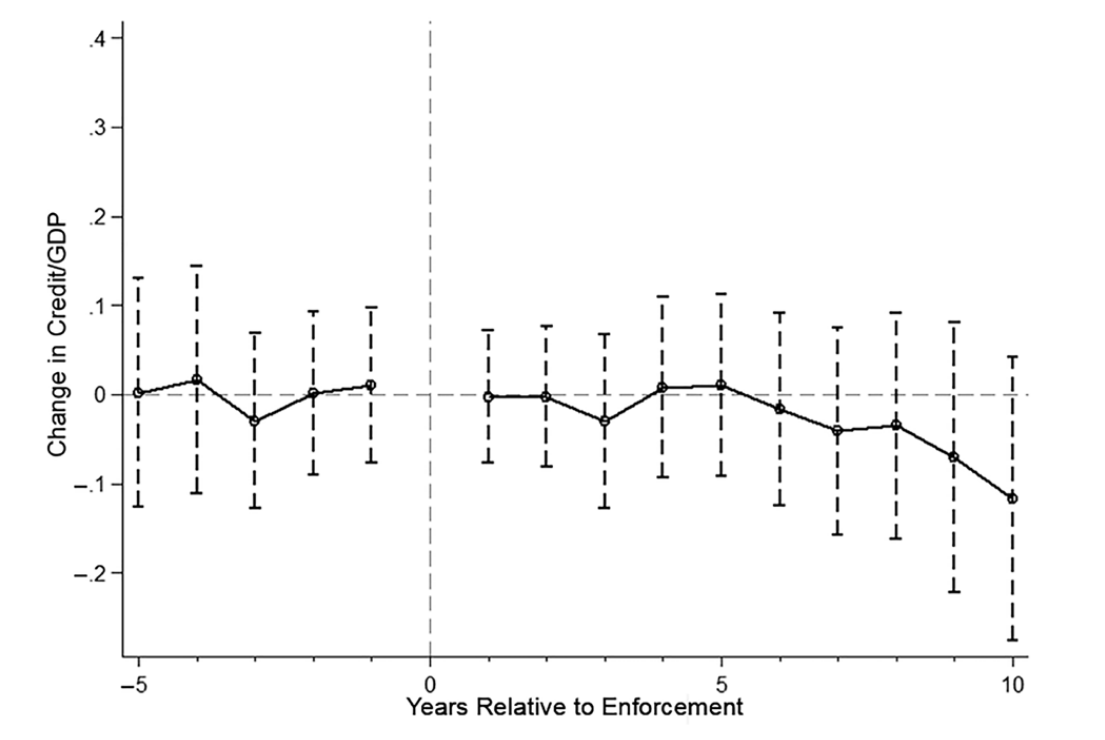
\includegraphics[width=\textwidth]{images/dynamic_orig_credit}
        \caption{Credit}
    \end{subfigure}
    \caption{Dynamic Effects on Citation Weight, Stock Market Capitalization, Trade and Credit}
    \label{fig:dynamic_orig}
\end{figure}

    \pagebreak

    \section{Extension}\label{sec:extension}
    The approach taken by the authors for both the baseline and the industry-level study may be considered naive and outdated: as previously treated units are included in the subsequent control groups, the resulting estimate for the $\alpha_1$`s and $\beta_1$`s is a weighted average of the treatment effects for each group, with weights that may even be negative, and thus potentially biased.
To address this issue, I adopt a modern diff-in-diff technique proposed by~\textcite{callaway}, implemented in Stata in the \texttt{csdid} package.
It offers two primary advantages:
\begin{enumerate}
\item Enhanced Control Group Selection: It provides flexibility in choosing control groups.
Specifically, it allows to utilize \textit{not-yet treated units} as controls in addition to \textit{never-treated} units (as this dataset lacks never treated groups).
\item Covariate Incorporation: it accommodates the inclusion of covariates, thereby ensuring that the parallel conditions assumption holds conditionally on these covariates, and implicitly handling the fixed effects.
\end{enumerate}
In particular, I focus on evaluating the average treatment effect (ATT) by treatment group, reported in~\ref{tab:group}.
Moreover, I reproduce, in figure~\ref{fig:dynamic_att} the dynamics in the $(-5,10)$ year window around the enforcement year.

\subsection{Treatment Effect by Group}\label{subsec:staggered-treatment-estimate}
Table~\ref{tab:group} and its graphical representation in figure~\ref{fig:group_att} reproduce the average treatment effect for different groups, using the industry-level dataset.
A similar analysis has been performed on the country level dataset, and in both cases, the treatment effect are found to be not statistically relevant.

\begin{figure}[h!]
    \centering

    \begin{subfigure}[b]{0.40\textwidth}
        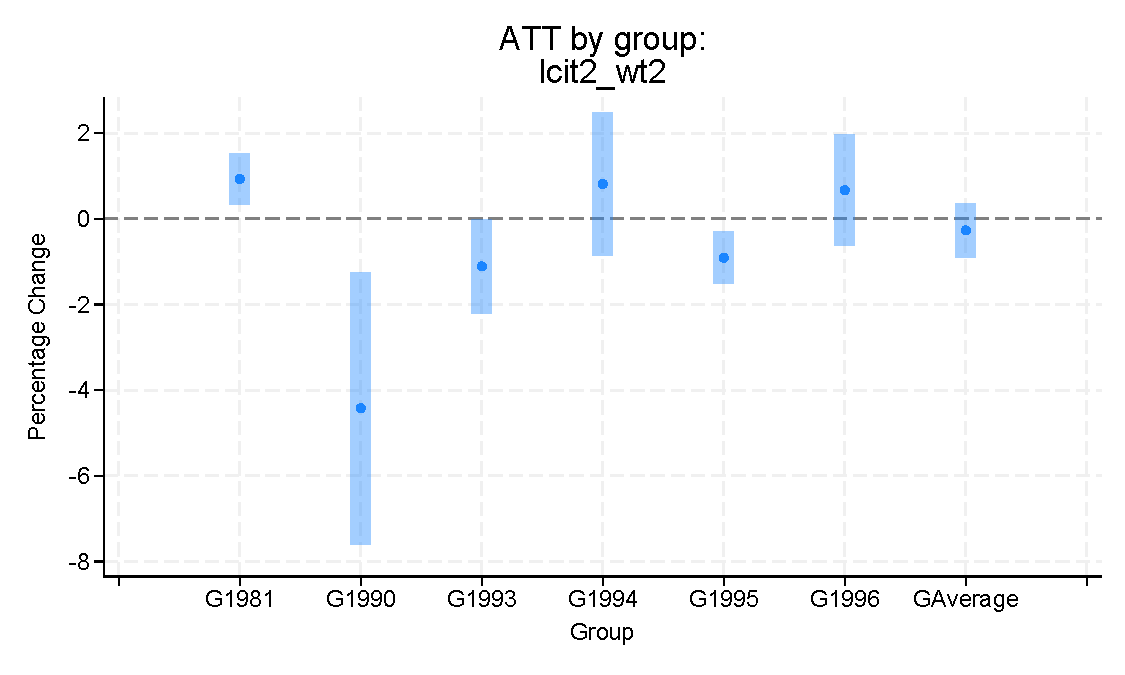
\includegraphics[width=\linewidth]{images/group_lcit2_wt2}
        \caption{Citation Weight}
    \end{subfigure}
    \hfill
    \begin{subfigure}[b]{0.40\textwidth}
        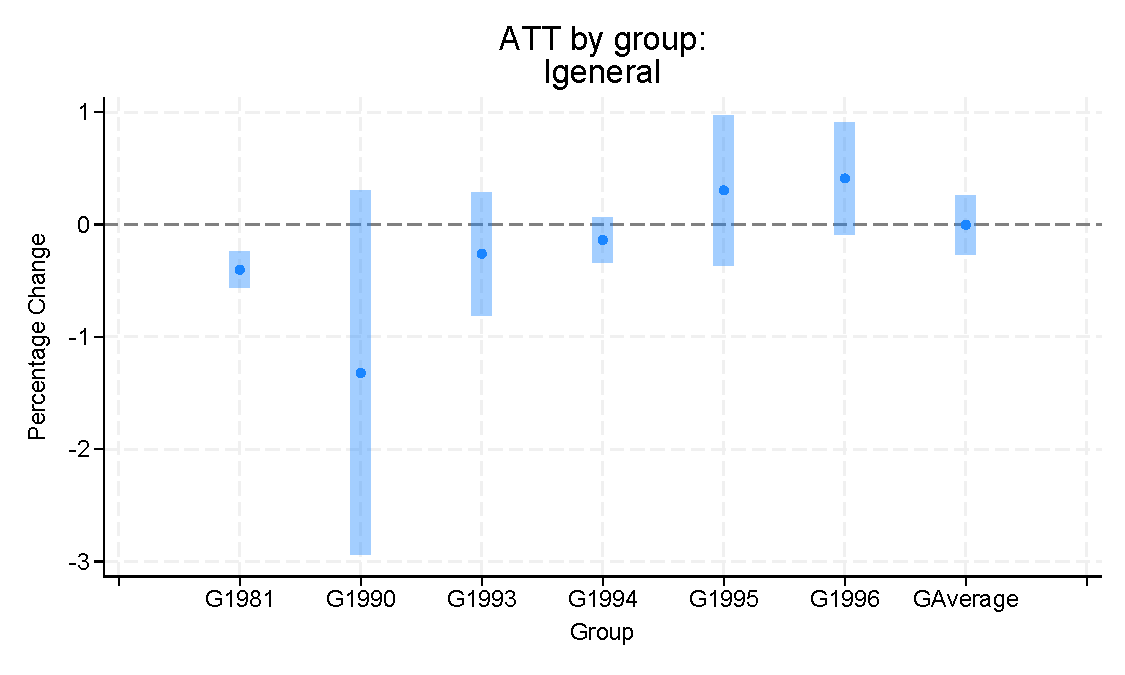
\includegraphics[width=\linewidth]{images/group_lgeneral}
        \caption{General Innovation}
    \end{subfigure}

    \vspace{0.4cm}

    \begin{subfigure}[b]{0.40\textwidth}
        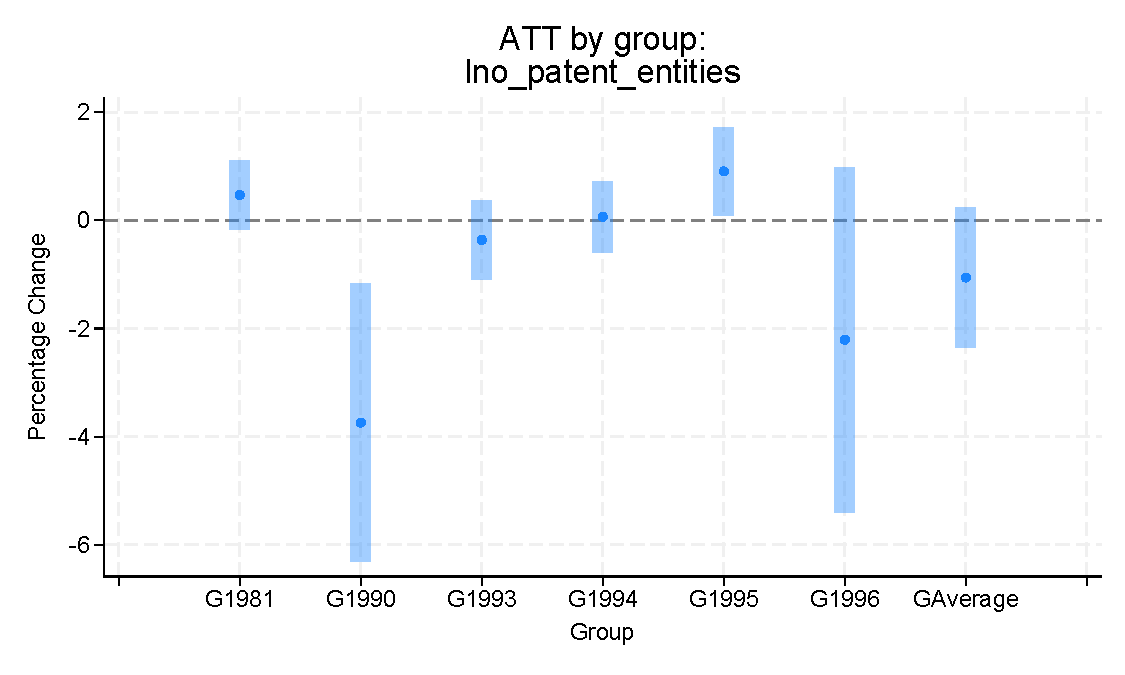
\includegraphics[width=\linewidth]{images/group_lno_patent_entities}
        \caption{Patent Entities}
    \end{subfigure}
    \hfill
    \begin{subfigure}[b]{0.45\textwidth}
        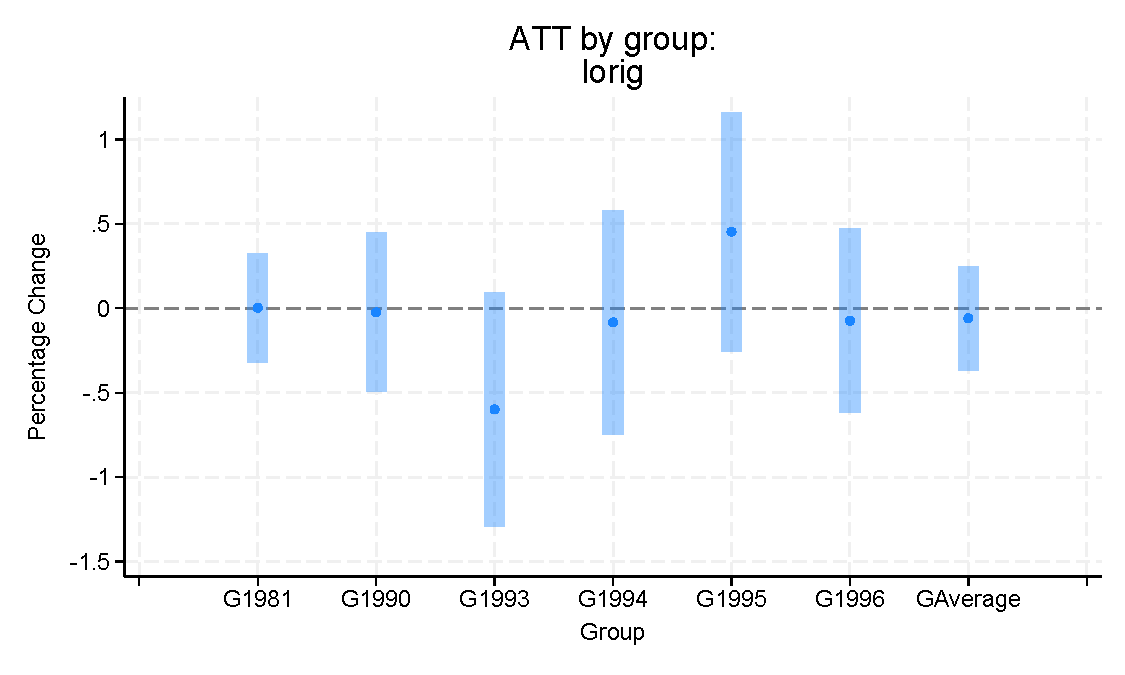
\includegraphics[width=\linewidth]{images/group_lorig}
        \caption{Originality}
    \end{subfigure}

    \vspace{0.4cm}

    \begin{subfigure}[b]{0.40\textwidth}
        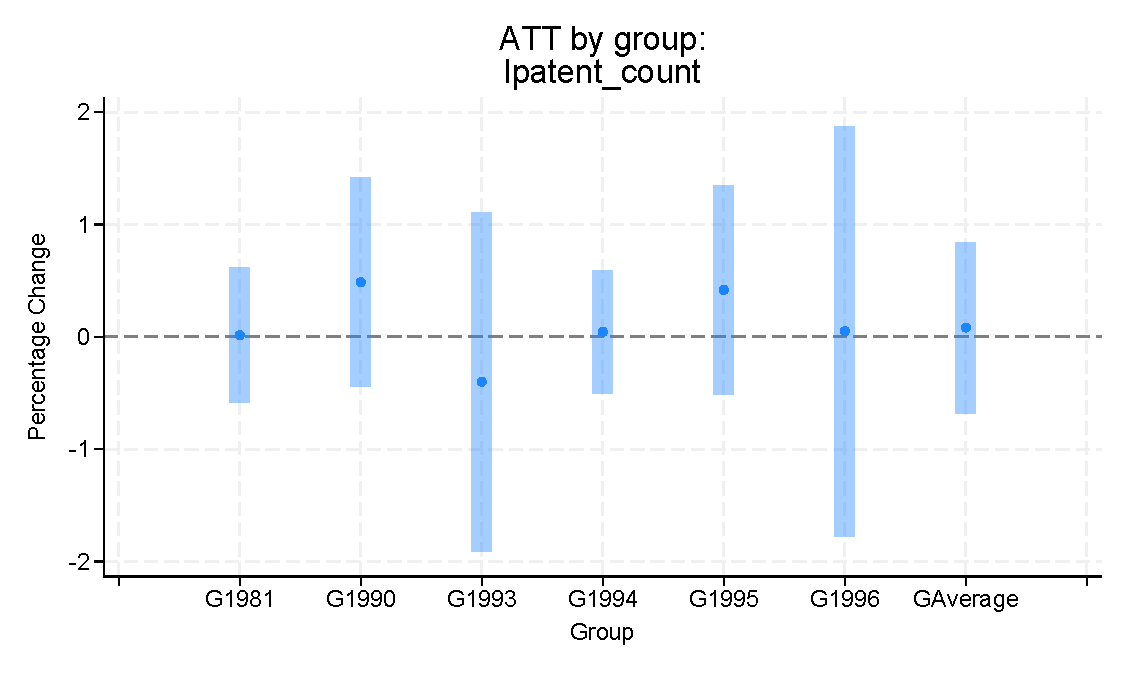
\includegraphics[width=\linewidth]{images/group_lpatent_count}
        \caption{Patent Count}
    \end{subfigure}
    \hfill
    \begin{subfigure}[b]{0.40\textwidth}
        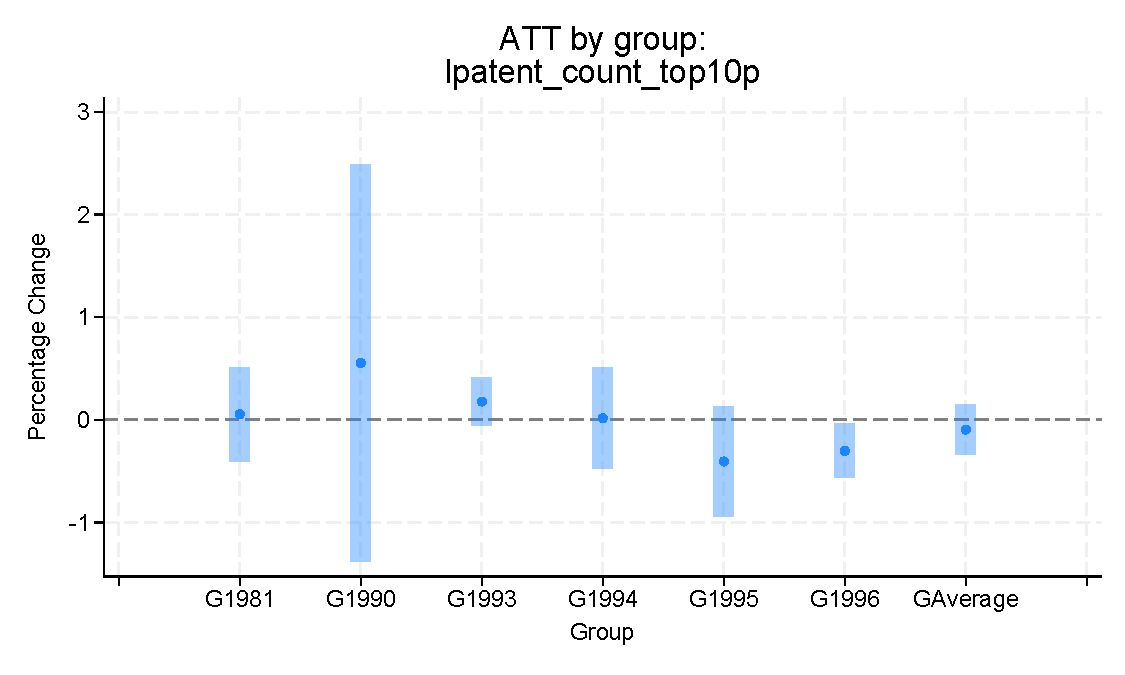
\includegraphics[width=\linewidth]{images/group_lpatent_count_top10p}
        \caption{Top 10\% Patents}
    \end{subfigure}

    \caption{ATT Estimates by Group Across Innovation Measures}
    \label{fig:group_att}
\end{figure}

\begin{landscape}
    \begin{table}[h!]
\centering
\caption{ATT by Group}
\label{tab:group}
\begin{tabular}{l*{6}{c}}
\hline\hline
                    &\multicolumn{1}{c}{(1)}&\multicolumn{1}{c}{(2)}&\multicolumn{1}{c}{(3)}&\multicolumn{1}{c}{(4)}&\multicolumn{1}{c}{(5)}&\multicolumn{1}{c}{(6)}\\
                    &\multicolumn{1}{c}{Patent Count}&\multicolumn{1}{c}{Patent Entities}&\multicolumn{1}{c}{Citation Weight}&\multicolumn{1}{c}{Top 10\% Patents}&\multicolumn{1}{c}{General Innovation}&\multicolumn{1}{c}{Originality}\\
\hline
GAverage            &      0.0823         &      -1.059         &      -0.270         &     -0.0946         &    -0.00366         &     -0.0588         \\
                    &     (0.388)         &     (0.657)         &     (0.326)         &     (0.124)         &     (0.134)         &     (0.157)         \\
[1em]
G1981               &      0.0141         &       0.469         &       0.933\sym{***}&      0.0542         &      -0.403\sym{***}&     0.00337         \\
                    &     (0.307)         &     (0.324)         &     (0.308)         &     (0.235)         &    (0.0810)         &     (0.165)         \\
[1em]
G1990               &       0.486         &      -3.740\sym{***}&      -4.424\sym{***}&       0.555         &      -1.322         &     -0.0240         \\
                    &     (0.473)         &     (1.310)         &     (1.618)         &     (0.987)         &     (0.826)         &     (0.241)         \\
[1em]
G1993               &      -0.400         &      -0.363         &      -1.111\sym{**} &       0.179         &      -0.262         &      -0.599\sym{*}  \\
                    &     (0.770)         &     (0.376)         &     (0.562)         &     (0.117)         &     (0.279)         &     (0.355)         \\
[1em]
G1994               &      0.0439         &      0.0655         &       0.814         &      0.0152         &      -0.138         &     -0.0832         \\
                    &     (0.281)         &     (0.335)         &     (0.857)         &     (0.251)         &     (0.103)         &     (0.338)         \\
[1em]
G1995               &       0.417         &       0.904\sym{**} &      -0.908\sym{***}&      -0.405         &       0.302         &       0.454         \\
                    &     (0.476)         &     (0.417)         &     (0.311)         &     (0.272)         &     (0.340)         &     (0.362)         \\
[1em]
G1996               &      0.0498         &      -2.207         &       0.668         &      -0.302\sym{**} &       0.409         &     -0.0736         \\
                    &     (0.930)         &     (1.626)         &     (0.659)         &     (0.135)         &     (0.254)         &     (0.278)         \\
\hline
Observations        &                     &                     &                     &                     &                     &                     \\
\hline\hline
\multicolumn{7}{l}{\footnotesize Standard errors in parentheses}\\
\multicolumn{7}{l}{\footnotesize \sym{*} \(p<0.10\), \sym{**} \(p<0.05\), \sym{***} \(p<0.01\)}\\
\end{tabular}
\end{table}


\end{landscape}


\subsection{Dynamics}\label{subsec:dynamics}
As reported in the following figure~\ref{fig:dynamic_att} and table~\ref{tab:dynamic_att}, also in the event aggregation of the $ATT(g,t)$ functions the effects are mostly statistically insignificant.

\begin{figure}[h!]
    \centering
    \begin{subfigure}[b]{0.45\textwidth}
        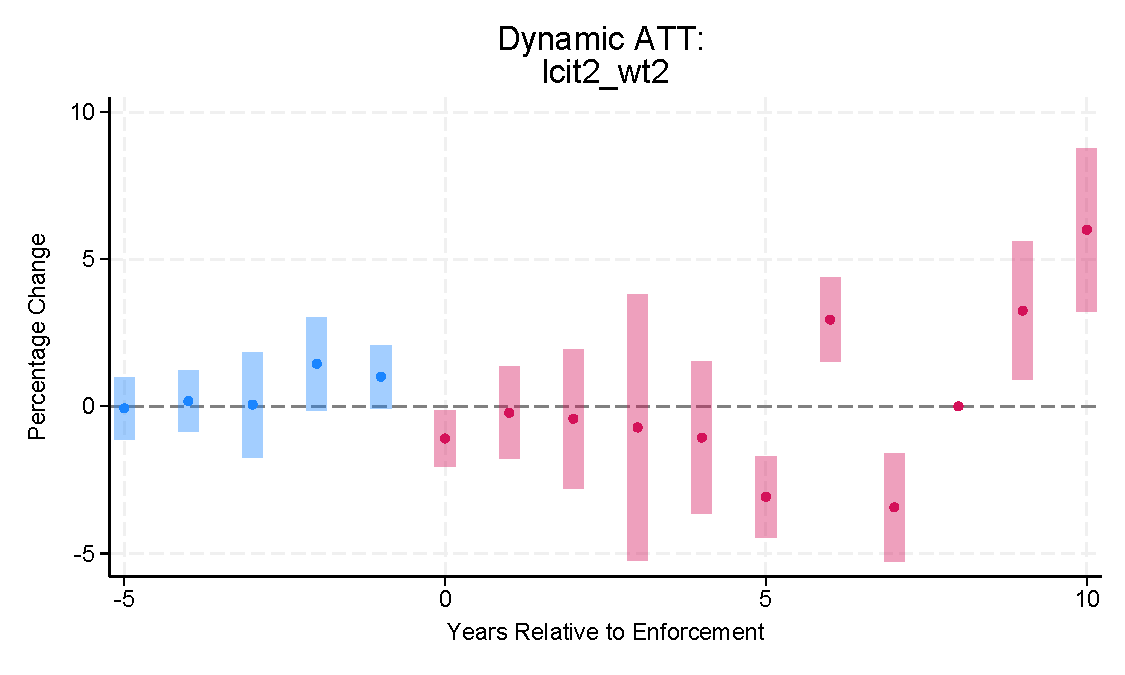
\includegraphics[width=\linewidth]{images/dynamic_att_lcit2_wt2}
        \caption{Citation Weight}
    \end{subfigure}
    \hfill
    \begin{subfigure}[b]{0.45\textwidth}
        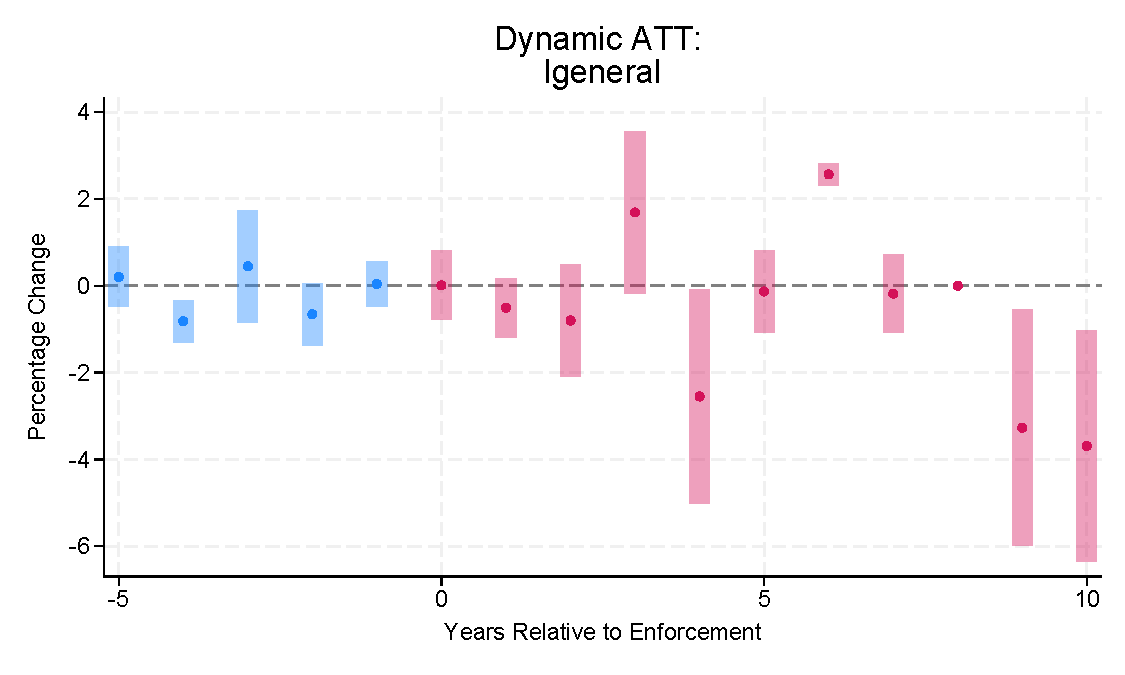
\includegraphics[width=\linewidth]{images/dynamic_att_lgeneral}
        \caption{General Innovation}
    \end{subfigure}

    \vspace{0.5cm}

    \begin{subfigure}[b]{0.45\textwidth}
        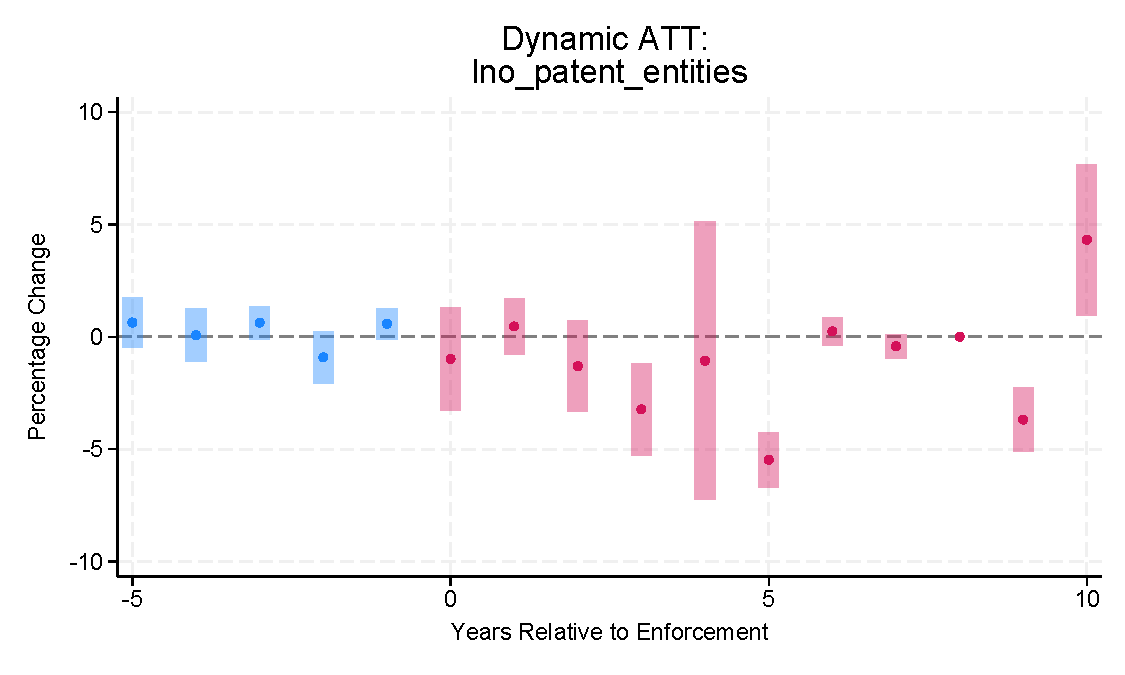
\includegraphics[width=\linewidth]{images/dynamic_att_lno_patent_entities}
        \caption{Patent Entities}
    \end{subfigure}
    \hfill
    \begin{subfigure}[b]{0.45\textwidth}
        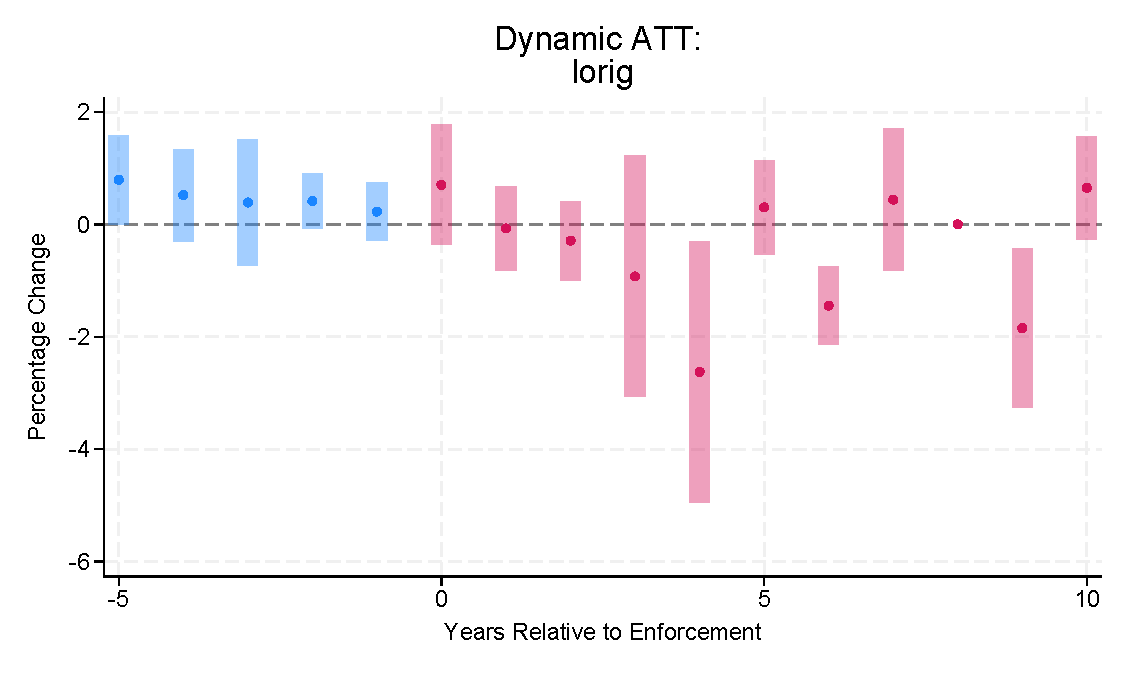
\includegraphics[width=\linewidth]{images/dynamic_att_lorig}
        \caption{Originality}
    \end{subfigure}

    \vspace{0.5cm}

    \begin{subfigure}[b]{0.45\textwidth}
        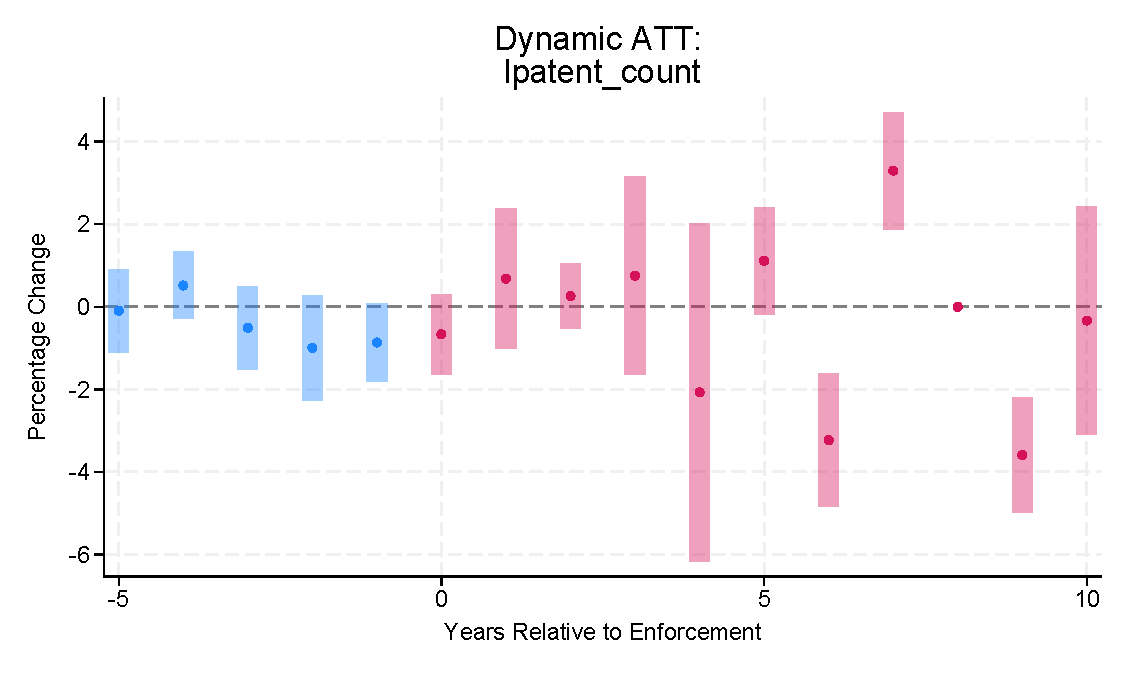
\includegraphics[width=\linewidth]{images/dynamic_att_lpatent_count}
        \caption{Patent Count}
    \end{subfigure}
    \hfill
    \begin{subfigure}[b]{0.45\textwidth}
        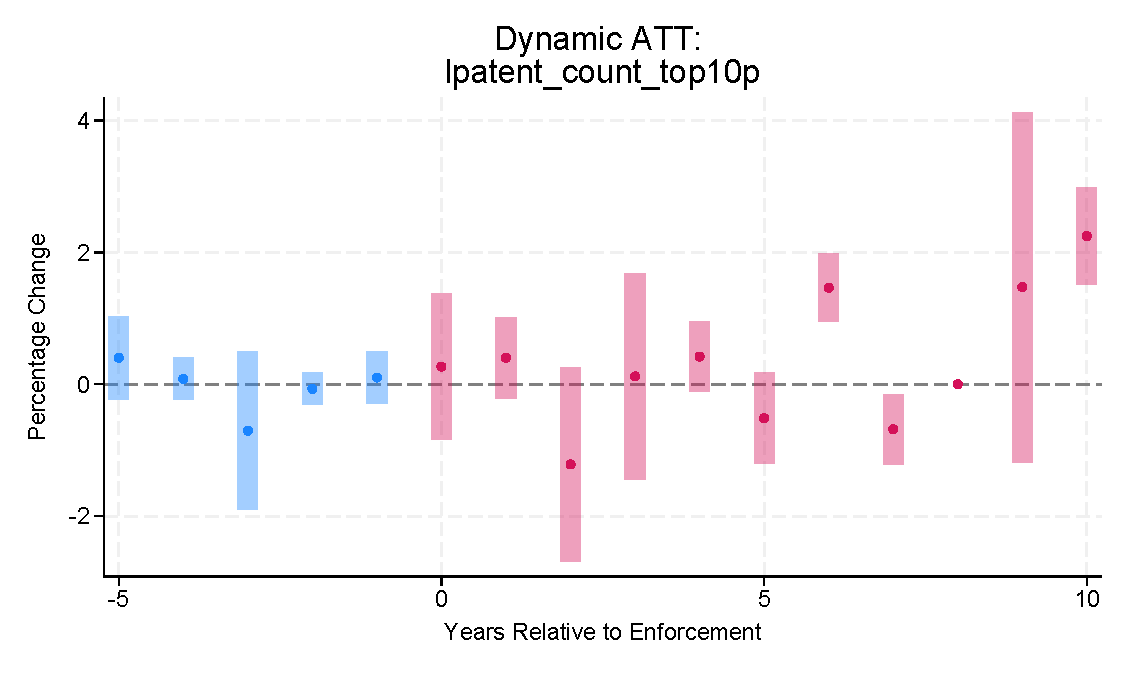
\includegraphics[width=\linewidth]{images/dynamic_att_lpatent_count_top10p}
        \caption{Top 10\% Patents}
    \end{subfigure}

    \caption{Dynamic ATT Estimates Across Innovation Measures}
    \label{fig:dynamic_att}
\end{figure}

\begin{landscape}
    \begin{longtable}{l*{6}{c}}
    \caption{Dynamic ATT by Event Time}
    \label{tab:dynamic_att} \\

\hline\hline
                    &\multicolumn{1}{c}{(1)}&\multicolumn{1}{c}{(2)}&\multicolumn{1}{c}{(3)}&\multicolumn{1}{c}{(4)}&\multicolumn{1}{c}{(5)}&\multicolumn{1}{c}{(6)}\\
                    &\multicolumn{1}{c}{Patent Count}&\multicolumn{1}{c}{Patent Entities}&\multicolumn{1}{c}{Citation Weight}&\multicolumn{1}{c}{Top 10\% Patents}&\multicolumn{1}{c}{General Innovation}&\multicolumn{1}{c}{Originality}\\
\hline
Pre\_avg            &      -0.389         &       0.199         &       0.523\sym{**} &     -0.0369         &      -0.157         &       0.470\sym{**} \\
                    &     (0.300)         &     (0.260)         &     (0.238)         &     (0.113)         &     (0.244)         &     (0.188)         \\
[1em]
Post\_avg           &           0         &           0         &           0         &           0         &           0         &           0         \\
                    &         (.)         &         (.)         &         (.)         &         (.)         &         (.)         &         (.)         \\
[1em]
Tm5                 &     -0.0947         &       0.635         &     -0.0709         &       0.402         &       0.203         &       0.795\sym{**} \\
                    &     (0.514)         &     (0.562)         &     (0.542)         &     (0.321)         &     (0.353)         &     (0.404)         \\
[1em]
Tm4                 &       0.517         &      0.0696         &       0.176         &      0.0820         &      -0.818\sym{***}&       0.521         \\
                    &     (0.414)         &     (0.598)         &     (0.526)         &     (0.163)         &     (0.246)         &     (0.417)         \\
[1em]
Tm3                 &      -0.508         &       0.631\sym{*}  &      0.0577         &      -0.703         &       0.447         &       0.391         \\
                    &     (0.516)         &     (0.374)         &     (0.910)         &     (0.610)         &     (0.659)         &     (0.574)         \\
[1em]
Tm2                 &      -0.995         &      -0.918         &       1.447\sym{*}  &     -0.0681         &      -0.657\sym{*}  &       0.416\sym{*}  \\
                    &     (0.646)         &     (0.598)         &     (0.809)         &     (0.122)         &     (0.365)         &     (0.248)         \\
[1em]
Tm1                 &      -0.864\sym{*}  &       0.576         &       1.007\sym{*}  &       0.102         &      0.0392         &       0.228         \\
                    &     (0.479)         &     (0.351)         &     (0.549)         &     (0.198)         &     (0.259)         &     (0.266)         \\
[1em]
Tp0                 &      -0.664         &      -0.982         &      -1.093\sym{**} &       0.267         &     0.00942         &       0.706         \\
                    &     (0.495)         &     (1.166)         &     (0.491)         &     (0.567)         &     (0.406)         &     (0.547)         \\
[1em]
Tp1                 &       0.683         &       0.459         &      -0.218         &       0.400         &      -0.507         &     -0.0711         \\
                    &     (0.869)         &     (0.639)         &     (0.802)         &     (0.312)         &     (0.349)         &     (0.381)         \\
[1em]
Tp2                 &       0.258         &      -1.308         &      -0.423         &      -1.215         &      -0.800         &      -0.290         \\
                    &     (0.401)         &     (1.034)         &     (1.206)         &     (0.751)         &     (0.663)         &     (0.359)         \\
[1em]
Tp3                 &       0.752         &      -3.226\sym{***}&      -0.720         &       0.120         &       1.688\sym{*}  &      -0.926         \\
                    &     (1.226)         &     (1.049)         &     (2.299)         &     (0.795)         &     (0.950)         &     (1.094)         \\
[1em]
Tp4                 &      -2.070         &      -1.072         &      -1.064         &       0.421         &      -2.550\sym{**} &      -2.626\sym{**} \\
                    &     (2.091)         &     (3.154)         &     (1.314)         &     (0.272)         &     (1.262)         &     (1.183)         \\
[1em]
Tp5                 &       1.115\sym{*}  &      -5.474\sym{***}&      -3.080\sym{***}&      -0.514         &      -0.133         &       0.302         \\
                    &     (0.663)         &     (0.620)         &     (0.709)         &     (0.350)         &     (0.476)         &     (0.423)         \\
[1em]
Tp6                 &      -3.230\sym{***}&       0.241         &       2.945\sym{***}&       1.464\sym{***}&       2.563\sym{***}&      -1.446\sym{***}\\
                    &     (0.821)         &     (0.311)         &     (0.728)         &     (0.263)         &     (0.130)         &     (0.356)         \\
[1em]
Tp7                 &       3.299\sym{***}&      -0.423         &      -3.436\sym{***}&      -0.682\sym{**} &      -0.181         &       0.441         \\
                    &     (0.724)         &     (0.272)         &     (0.938)         &     (0.269)         &     (0.463)         &     (0.647)         \\
[1em]
Tp8                 &           0         &           0         &           0         &           0         &           0         &           0         \\
                    &         (.)         &         (.)         &         (.)         &         (.)         &         (.)         &         (.)         \\
[1em]
Tp9                 &      -3.590\sym{***}&      -3.686\sym{***}&       3.249\sym{***}&       1.474         &      -3.271\sym{**} &      -1.847\sym{**} \\
                    &     (0.715)         &     (0.725)         &     (1.201)         &     (1.355)         &     (1.385)         &     (0.723)         \\
[1em]
Tp10                &      -0.333         &       4.320\sym{**} &       6.000\sym{***}&       2.248\sym{***}&      -3.692\sym{***}&       0.651         \\
                    &     (1.406)         &     (1.715)         &     (1.414)         &     (0.378)         &     (1.357)         &     (0.467)         \\
\hline
Observations        &                     &                     &                     &                     &                     &                     \\
\hline\hline
\multicolumn{7}{l}{\footnotesize Standard errors in parentheses}\\
\multicolumn{7}{l}{\footnotesize \sym{*} \(p<0.10\), \sym{**} \(p<0.05\), \sym{***} \(p<0.01\)}\\
\end{longtable}


\end{landscape}


\newpage

    \pagebreak

    \section{Conclusion}\label{sec:conclusion}
    The results of the paper do not seem to hold when confronted with more advanced DiD techniques, and the \texttt{csdid}-estimated ATT are mostly not statistically significant, both when aggregated by group and in the overall average.
    Therefore, we can conclude that enforcing insider trading laws alone is unlikely to have the large effect claimed by the authors, and other confounding effects may be at play.

    \printbibliography
\end{document}